\documentclass[tikz]{standalone}

\usepackage{libertinus}
\usepackage{tikz}
\usepackage{pgfplots}
\pgfplotsset{compat=1.18}

\begin{document}

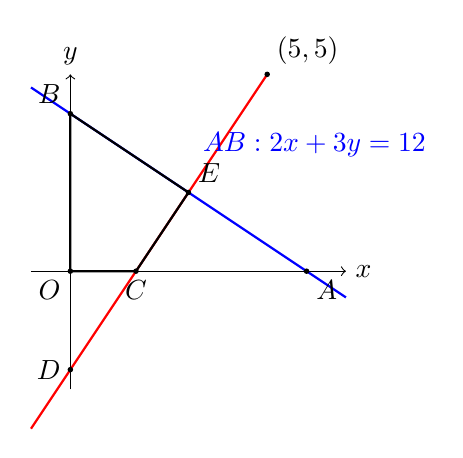
\begin{tikzpicture}[scale=0.5]

  % Axes
  \draw[->] (-1,0) -- (7,0) node[right] {$x$};
  \draw[->] (0,-3) -- (0,5) node[above] {$y$};

  % Key points
  \coordinate (O) at (0,0);
  \coordinate (A) at (6,0);
  \coordinate (B) at (0,4);
  \coordinate (C) at (5/3,0);
  \coordinate (D) at (0,-2.5);
  \coordinate (E) at (3,2);
  \coordinate (P) at (5,5);

  % Line AB: 2x + 3y = 12
  \draw[thick, blue, domain=-1:7] plot (\x,{(12-2*\x)/3});

  % Perpendicular line through (5,5): y = 3/2 x - 5/2
  \draw[thick, red, domain=-1:5] plot (\x,{1.5*\x - 2.5});

  % Triangle/polygon O-C-E-B
  \draw[thick] (O) -- (C) -- (E) -- (B) -- cycle;

  % Points
  \fill (O) circle (2pt) node[below left] {$O$};
  \fill (A) circle (2pt) node[below right] {$A$};
  \fill (B) circle (2pt) node[above left] {$B$};
  \fill (C) circle (2pt) node[below] {$C$};
  \fill (D) circle (2pt) node[left] {$D$};
  \fill (E) circle (2pt) node[above right] {$E$};
  \fill (P) circle (2pt) node[above right] {$(5,5)$};

  % Labels for lines
  \node[blue] at (6.2,3.2) {$AB: 2x+3y=12$};

\end{tikzpicture}

\end{document}
